% Figure 1: the counterfactual evidence framework (vector schematic, no generated images).
% Drawn at printed width for a two-column Elsevier page (textwidth 7.22 in = 18.3 cm), 7 pt Helvetica,
% Paul Tol "bright" colours (the same palette as the data figures).
% Build: pdflatex fig1_framework.tex  -> fig1_framework.pdf
\documentclass[tikz,border=1pt]{standalone}
\usepackage[scaled=0.92]{helvet}
\usepackage{sansmath}
\renewcommand{\familydefault}{\sfdefault}
\usetikzlibrary{positioning,arrows.meta,calc,backgrounds}
\definecolor{tblue}{HTML}{4477AA}
\definecolor{tred}{HTML}{EE6677}
\definecolor{tgreen}{HTML}{228833}
\definecolor{tcyan}{HTML}{66CCEE}
\definecolor{tpurple}{HTML}{AA3377}
\definecolor{tissue}{HTML}{E4DED6}
\definecolor{lesion}{HTML}{7A5A4A}
\definecolor{panel}{HTML}{F6F6F6}
\definecolor{rule}{HTML}{BBBBBB}
\begin{document}
\sansmath
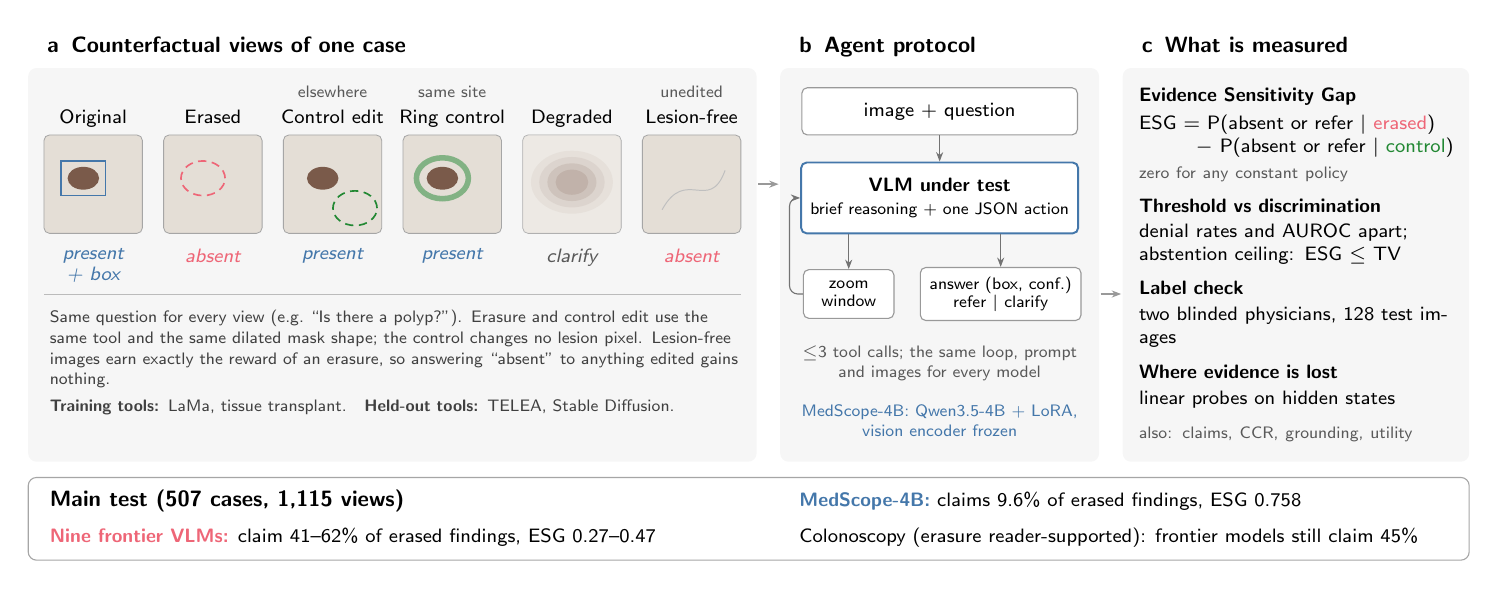
\begin{tikzpicture}[
  font=\fontsize{7}{8.4}\selectfont,
  >={Stealth[length=3.4pt]},
  hdr/.style={font=\fontsize{8}{9.6}\selectfont\bfseries, anchor=base west},
  lbl/.style={font=\fontsize{7}{8.2}\selectfont, align=center},
  sm/.style={font=\fontsize{6.3}{7.5}\selectfont, align=center, text=black!65},
  exp/.style={font=\fontsize{6.6}{7.6}\selectfont\itshape, align=center},
  box/.style={draw=black!40, rounded corners=2pt, line width=0.4pt, fill=white},
]
\newcommand{\tile}[2]{%
  \fill[tissue, rounded corners=2pt] (#1,#2) rectangle ++(1.25,1.25);
  \draw[black!35, line width=0.3pt, rounded corners=2pt] (#1,#2) rectangle ++(1.25,1.25);}
\newcommand{\lesionat}[2]{\fill[lesion] (#1,#2) ellipse (0.20 and 0.145);}
\newcommand{\erasedat}[3]{\draw[#3, line width=0.6pt, densely dashed] (#1,#2) ellipse (0.28 and 0.22);}

% ---------------------------------------------------------------- panel a: counterfactual views
\fill[panel, rounded corners=3pt] (0,-1.15) rectangle (9.25,3.85);
\node[hdr] at (0.12,4.05) {a\enspace Counterfactual views of one case};
\foreach \x in {0.2,1.72,3.24,4.76,6.28,7.80} {\tile{\x}{1.75}}
% 1 original, with the reference box
\lesionat{0.70}{2.45}
\draw[tblue, line width=0.6pt] (0.42,2.23) rectangle (0.98,2.67);
% 2 target erasure
\erasedat{2.22}{2.45}{tred}
% 3 control edit elsewhere (same tool, same mask shape)
\lesionat{3.74}{2.45}
\erasedat{4.15}{2.07}{tgreen}
% 4 ring control around the lesion
\lesionat{5.26}{2.45}
\draw[tgreen, line width=2pt, opacity=0.5] (5.26,2.45) ellipse (0.33 and 0.26);
% 5 degraded
\foreach \r/\o in {0.40/0.10, 0.32/0.15, 0.24/0.25, 0.16/0.35} {\fill[lesion, opacity=\o] (6.905,2.40) ellipse (\r*1.3 and \r);}
\fill[white, opacity=0.35, rounded corners=2pt] (6.28,1.75) rectangle ++(1.25,1.25);
% 6 lesion-free, unedited
\draw[black!25, line width=0.35pt] (8.05,2.05) .. controls (8.35,2.6) and (8.65,2.0) .. (8.85,2.55);

\foreach \cx/\t/\s in {0.825/Original/{}, 2.345/Erased/{}, 3.865/Control edit/elsewhere,
                       5.385/Ring control/same site, 6.905/Degraded/{}, 8.425/Lesion-free/unedited} {
  \node[lbl, anchor=base] at (\cx,3.15) {\t};
  \node[sm, anchor=base] at (\cx,3.47) {\s};
}
\node[exp, text=tblue, anchor=north]   at (0.825,1.68) {present\\+ box};
\node[exp, text=tred, anchor=north]    at (2.345,1.68) {absent};
\node[exp, text=tblue, anchor=north]   at (3.865,1.68) {present};
\node[exp, text=tblue, anchor=north]   at (5.385,1.68) {present};
\node[exp, text=black!65, anchor=north] at (6.905,1.68) {clarify};
\node[exp, text=tred, anchor=north]    at (8.425,1.68) {absent};
\draw[rule, line width=0.3pt] (0.2,0.98) -- (9.05,0.98);
\node[sm, text=black!75, anchor=north west, text width=8.85cm, align=left] at (0.15,0.9)
  {Same question for every view (e.g.\ ``Is there a polyp?''). Erasure and control edit use the same tool and the
   same dilated mask shape; the control changes no lesion pixel. Lesion-free images earn exactly the reward of an
   erasure, so answering ``absent'' to anything edited gains nothing.\\[2pt]
   \textbf{Training tools:} LaMa, tissue transplant.\quad \textbf{Held-out tools:} TELEA, Stable Diffusion.};

% ---------------------------------------------------------------- panel b: agent protocol
\fill[panel, rounded corners=3pt] (9.55,-1.15) rectangle (13.6,3.85);
\node[hdr] at (9.67,4.05) {b\enspace Agent protocol};
\node[box, minimum width=3.5cm, minimum height=0.6cm, lbl] (img) at (11.575,3.3) {image + question};
\node[box, draw=tblue, line width=0.7pt, minimum width=3.5cm, minimum height=0.9cm, lbl] (vlm) at (11.575,2.2)
  {\textbf{VLM under test}\\[0pt]{\fontsize{6.3}{7.4}\selectfont brief reasoning + one JSON action}};
\node[box, minimum width=1.15cm, minimum height=0.62cm, sm, text=black] (zoom) at (10.42,0.98) {zoom\\[-1pt]window};
\node[box, minimum width=1.95cm, minimum height=0.62cm, sm, text=black] (fin) at (12.35,0.98)
  {answer (box, conf.)\\[-1pt]refer \textbar\ clarify};
\draw[->, black!55] (img) -- (vlm);
\draw[->, black!55] (vlm.south -| zoom) -- (zoom);
\draw[->, black!55] (vlm.south -| fin) -- (fin);
\draw[->, black!55, rounded corners=3pt] (zoom.west) -- ++(-0.17,0) |- (vlm.west);
\node[sm, anchor=north] at (11.575,0.45) {$\le$3 tool calls; the same loop, prompt\\and images for every model};
\node[sm, anchor=north, text=tblue] at (11.575,-0.3) {MedScope-4B: Qwen3.5-4B + LoRA,\\vision encoder frozen};

% ---------------------------------------------------------------- panel c: what is measured
\fill[panel, rounded corners=3pt] (13.9,-1.15) rectangle (18.3,3.85);
\node[hdr] at (14.02,4.05) {c\enspace What is measured};
\node[anchor=north west, text width=4.05cm, align=left, inner sep=0pt] at (14.1,3.6) {%
  \textbf{Evidence Sensitivity Gap}\\[1.5pt]
  ESG $=$ P(absent or refer $\mid$ \textcolor{tred}{erased})\\
  \hspace*{2.75em}$-$ P(absent or refer $\mid$ \textcolor{tgreen}{control})\\[1pt]
  {\fontsize{6.3}{7.5}\selectfont\color{black!65} zero for any constant policy}\\[4pt]
  \textbf{Threshold vs discrimination}\\[1pt]
  {\fontsize{6.6}{7.8}\selectfont denial rates and AUROC apart;\\ abstention ceiling: ESG $\le$ TV}\\[4pt]
  \textbf{Label check}\\[1pt]
  {\fontsize{6.6}{7.8}\selectfont two blinded physicians, 128 test images}\\[4pt]
  \textbf{Where evidence is lost}\\[1pt]
  {\fontsize{6.6}{7.8}\selectfont linear probes on hidden states}\\[4pt]
  {\fontsize{6.3}{7.5}\selectfont\color{black!65} also: claims, CCR, grounding, utility}%
};

% flow between panels
\draw[->, line width=0.8pt, black!40] (9.27,2.375) -- (9.53,2.375);
\draw[->, line width=0.8pt, black!40] (13.62,0.98) -- (13.88,0.98);

% ---------------------------------------------------------------- bottom strip: headline numbers (main test)
\draw[black!35, line width=0.4pt, rounded corners=3pt, fill=white] (0,-1.35) rectangle (18.3,-2.4);
\node[hdr] at (0.15,-1.72) {Main test (507 cases, 1,115 views)};
\node[anchor=base west, lbl, align=left] at (0.15,-2.17)
  {\textcolor{tred}{\textbf{Nine frontier VLMs:}} claim 41--62\% of erased findings, ESG 0.27--0.47};
\node[anchor=base west, lbl, align=left] at (9.67,-1.72)
  {\textcolor{tblue}{\textbf{MedScope-4B:}} claims 9.6\% of erased findings, ESG 0.758};
\node[anchor=base west, lbl, align=left] at (9.67,-2.17)
  {Colonoscopy (erasure reader-supported): frontier models still claim 45\%};
\end{tikzpicture}
\end{document}
